\documentclass[aspectratio=169,10pt]{beamer}

\usepackage[utf8]{inputenc}
\usepackage[T1]{fontenc}
\usepackage{lmodern}
\usepackage{amsmath,amssymb}
\usepackage{booktabs}
\usepackage{tabularx}
\usepackage{graphicx}
\usepackage{xcolor}
\usepackage{tcolorbox}
\usepackage{tikz}

% -------------------------------------------------------------
% COLOR DEFINITIONS (Strict Ivory & Charcoal Palette)
% -------------------------------------------------------------
\definecolor{bgivory}{HTML}{FAF8F5}
\definecolor{cardbg}{HTML}{FFFFFF}
\definecolor{charcoal}{HTML}{121316}
\definecolor{mutedgray}{HTML}{4A4B4E}
\definecolor{bordergray}{HTML}{E2DFD8}
\definecolor{airtelred}{HTML}{C8102E}
\definecolor{softgray}{HTML}{F4F2EC}
\definecolor{successgreen}{HTML}{1E6B38}

% Currency command (safe in pdfTeX)
\newcommand{\inr}{\text{Rs.\ }}

% -------------------------------------------------------------
% BEAMER THEME & GEOMETRY
% -------------------------------------------------------------
\setbeamersize{text margin left=6mm,text margin right=6mm}
\setbeamercolor{background canvas}{bg=bgivory}
\setbeamercolor{normal text}{fg=charcoal}
\setbeamercolor{frametitle}{fg=charcoal,bg=bgivory}
\setbeamercolor{structure}{fg=charcoal}
\setbeamerfont{frametitle}{size=\normalsize,series=\bfseries}
\setbeamertemplate{navigation symbols}{}

% Frame Title Template
\setbeamertemplate{frametitle}{%
  \vspace{0.08cm}%
  \noindent\begin{minipage}{\textwidth}%
    {\fontsize{9.5pt}{11.5pt}\selectfont\textbf{\insertframetitle}} \hfill {\fontsize{6.2pt}{7.5pt}\selectfont\textcolor{mutedgray}{\insertframesubtitle}}\\[0.04cm]%
    \textcolor{bordergray}{\rule{\textwidth}{0.35pt}}%
  \end{minipage}%
  \vspace{-0.22cm}%
}

% Footline Template
\setbeamertemplate{footline}{%
  \noindent\hspace*{6mm}\begin{minipage}{\dimexpr\paperwidth-12mm\relax}%
    \textcolor{bordergray}{\rule{\linewidth}{0.35pt}}\\[0.03cm]%
    {\fontsize{5.2pt}{6.5pt}\selectfont\textcolor{mutedgray}{Airtel Sync 2026 $\cdot$ Digital Track (Enterprise Track A) $\mid$ Project Udyam Digital}}%
    \hfill%
    {\fontsize{5.2pt}{6.5pt}\selectfont\textcolor{mutedgray}{\textbf{Team Neural Nexus} (YK, HR)}}%
    \hfill%
    {\fontsize{5.2pt}{6.5pt}\selectfont\textbf{Slide \insertframenumber{} of 7}}%
  \end{minipage}%
  \vspace{0.05cm}%
}

% Custom TColorBox Styles
\tcbset{
  academicbox/.style={
    colback=cardbg,
    colframe=bordergray,
    coltext=charcoal,
    arc=0.8mm,
    boxrule=0.35pt,
    left=1.5mm,
    right=1.5mm,
    top=0.8mm,
    bottom=0.8mm,
    boxsep=0pt
  },
  accentbox/.style={
    colback=softgray,
    colframe=bordergray,
    coltext=charcoal,
    arc=0.8mm,
    boxrule=0.35pt,
    left=1.5mm,
    right=1.5mm,
    top=0.8mm,
    bottom=0.8mm,
    boxsep=0pt
  }
}

\begin{document}

% =============================================================
% SLIDE 1: TITLE & EXECUTIVE VISION (The Single-Sitting Paradigm)
% =============================================================
\begin{frame}[plain]
  \vspace{0.25cm}
  \begin{center}
    {\fontsize{6.8pt}{8pt}\selectfont\textbf{\textcolor{airtelred}{AIRTEL SYNC 2026 $\cdot$ DIGITAL TRACK (ENTERPRISE TRACK A)}}} \\[0.12cm]
    {\fontsize{15pt}{18pt}\selectfont\textbf{Project Udyam Digital}} \\[0.08cm]
    {\fontsize{9pt}{11pt}\selectfont\textcolor{mutedgray}{Making 6 Crore+ Indian MSMEs Go Digital in One Sitting}} \\[0.04cm]
    {\fontsize{6.5pt}{7.8pt}\selectfont\textcolor{mutedgray}{Autonomous Neuro-Symbolic CPQ, Instant DPDP KYC \& Multi-Site Orchestration}} \\[0.15cm]
    \textcolor{bordergray}{\rule{0.8\paperwidth}{0.4pt}} \\[0.15cm]
  \end{center}

  \begin{columns}[T]
    \begin{column}{0.48\textwidth}
      \begin{tcolorbox}[academicbox, title={\fontsize{6.8pt}{8pt}\selectfont\textbf{\textcolor{charcoal}{The Enterprise MSME Acquisition Bottleneck}}}, coltitle=charcoal]
        {\fontsize{6.0pt}{7.2pt}\selectfont
        \begin{itemize}\setlength{\itemsep}{1pt}
          \item \textbf{Massive TAM with Low Penetration:} Accel Business dominates large enterprises but serves $<10\%$ of India's 63M MSMEs (Kiranas, clinics, CA firms, workshops).
          \item \textbf{17.6-Day Manual Sales Ordeal:} Journey relies on physical sales rep visits, 3--5 day PDF quoting lags, and 3.2 customer status chase calls.
          \item \textbf{The 56.4\% Quoting Drop-off:} Prospective owners drop off while awaiting cryptic enterprise quotes, defecting to fragmented local unmanaged ISPs.
          \item \textbf{Crippling CAC Burden:} Blended acquisition cost of \textbf{\inr 15,000} against a median monthly ARPU of \inr 6,900 (\inr 2,500 for micro-retail).
        \end{itemize}
        }
      \end{tcolorbox}
    \end{column}

    \begin{column}{0.48\textwidth}
      \begin{tcolorbox}[accentbox, title={\fontsize{6.8pt}{8pt}\selectfont\textbf{\textcolor{charcoal}{The Single-Sitting Breakthrough Solution}}}, coltitle=charcoal]
        {\fontsize{6.0pt}{7.2pt}\selectfont
        \begin{itemize}\setlength{\itemsep}{1pt}
          \item \textbf{$<$15-Minute Mobile Self-Serve:} Multi-turn conversational advisor in 10 Indic languages translating ambiguous merchant needs into deterministic quotes.
          \item \textbf{GST-Free Udyam Onboarding:} Unlocks 3.5 Crore unregistered MSMEs (historically 2.0\% conversion) via composite declaration rules.
          \item \textbf{DPDP Act 2023 Compliant:} Zero-persistence in-memory PII masking, cryptographic SHA-256 byte caching, and tamper-evident audit trails.
          \item \textbf{Deployed Production Monolith:} Fully functional on AWS EC2 (\texttt{http://65.1.112.251}) with 37/37 Pytest test suite verified.
        \end{itemize}
        }
      \end{tcolorbox}
    \end{column}
  \end{columns}

  \vspace{0.2cm}
  \begin{center}
    {\fontsize{6.0pt}{7.2pt}\selectfont
    \textbf{Team Neural Nexus:} YK $\cdot$ HR (Hrushikesh Ramilla) \quad $\vert$ \quad
    \textbf{Live Deployment:} \texttt{http://65.1.112.251} \quad $\vert$ \quad
    \textbf{GitHub:} \texttt{Hrushikesh-ramilla/project-udyam-digital}
    }
  \end{center}
\end{frame}

% =============================================================
% SLIDE 2: PROBLEM & 5,000-LEAD SMB FUNNEL BLEED DISSECTION
% =============================================================
\begin{frame}{Problem Statement \& Funnel Bleed Dissection}{Empirical Analysis of 5,000 SMB Leads (smb\_leads.csv, Apr--Jun 2026)}
  \begin{columns}[T]
    \begin{column}{0.51\textwidth}
      \begin{tcolorbox}[academicbox, title={\fontsize{6.5pt}{7.8pt}\selectfont\textbf{SMB Acquisition Funnel Degradation ($N = 5{,}000$)}}, coltitle=charcoal]
        \centering
        {\fontsize{5.2pt}{6.4pt}\selectfont
        \setlength{\tabcolsep}{3pt}
        \begin{tabularx}{\linewidth}{lrrr}
          \toprule
          \textbf{Funnel Stage} & \textbf{Leads} & \textbf{Stage \%} & \textbf{Cumulative \%} \\
          \midrule
          Leads Generated & 5,000 & 100.0\% & 100.0\% \\
          Contacted Outreach & 3,406 & 68.1\% & 68.1\% \\
          Needs Assessed (Field Visit) & 1,974 & 58.0\% & 39.5\% \\
          \textbf{Quote Accepted (Steepest Drop)} & \textbf{861} & \textbf{43.6\%} & \textbf{17.2\%} \\
          KYC Completed & 588 & 68.3\% & 11.8\% \\
          \textbf{Activated Customers} & \textbf{368} & \textbf{62.6\%} & \textbf{7.36\%} \\
          \bottomrule
        \end{tabularx}
        }
        \vspace{0.04cm}
        \begin{center}
          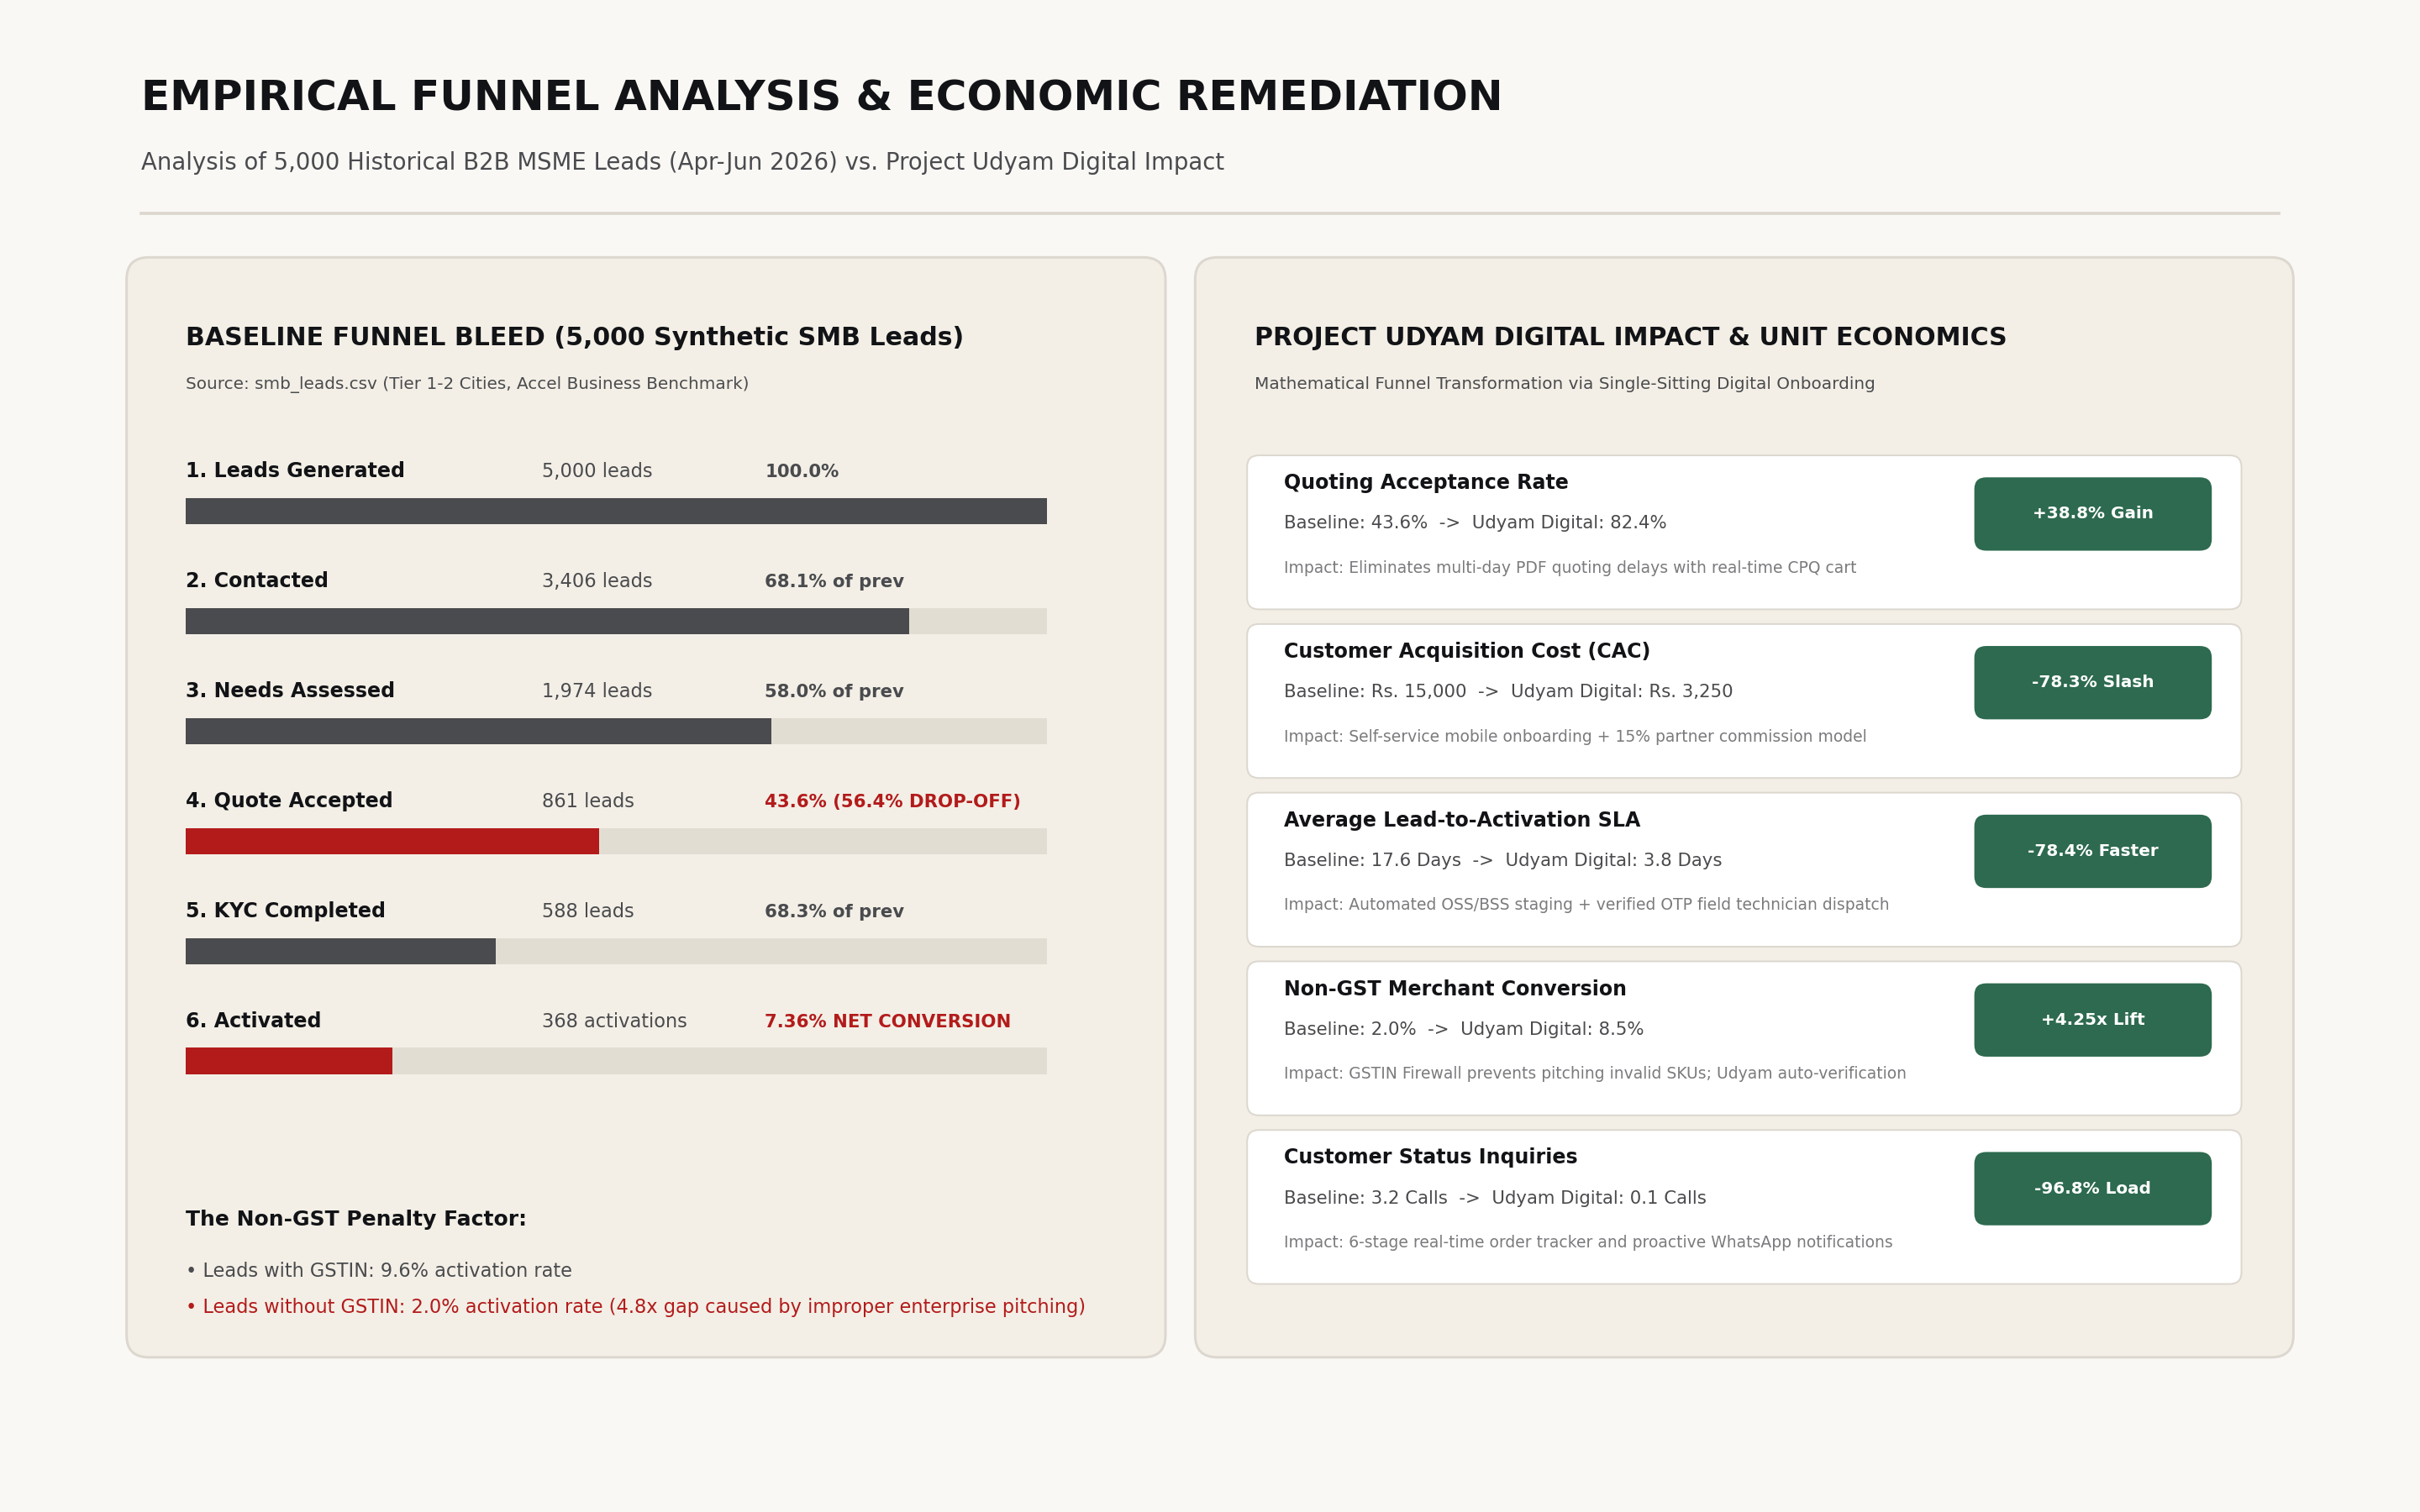
\includegraphics[width=0.96\linewidth,height=1.15cm,keepaspectratio]{assets/udyam-funnel-economics.png}
        \end{center}
      \end{tcolorbox}
    \end{column}

    \begin{column}{0.46\textwidth}
      \begin{tcolorbox}[academicbox, title={\fontsize{6.5pt}{7.8pt}\selectfont\textbf{The Three Structural Failure Modes}}, coltitle=charcoal]
        {\fontsize{5.5pt}{6.6pt}\selectfont
        \textbf{1. The 3--5 Day Quoting Abyss (56.4\% Drop)} \\
        Manual pricing and complex product codes create an intolerable latency gap. 1,113 of 1,974 assessed prospects abandon the pipeline while awaiting quotes. \\[0.06cm]
        \textbf{2. The Non-GST Regulatory Wall (4.8x Penalty)} \\
        Leads with active GSTIN activate at \textbf{9.6\%}; leads without GSTIN drop to \textbf{2.0\%}. 55\% of India's micro-enterprises operate below GST thresholds and are discarded by legacy KYC. \\[0.06cm]
        \textbf{3. Crippling Unit Economics (\inr 15k CAC)} \\
        A 17.6-day lead-to-activation cycle and 3.2 manual follow-up calls consume \inr 15,000 in direct sales acquisition costs against an \inr 6,900 median monthly revenue.
        }
      \end{tcolorbox}

      \vspace{0.04cm}
      \begin{tcolorbox}[accentbox]
        {\fontsize{5.4pt}{6.5pt}\selectfont
        \textbf{\textcolor{airtelred}{Target Mandate:}} Compress quote time from 5 days to $<60$ seconds, eliminate the non-GST drop-off via Udyam lookup, and automate status tracking.
        }
      \end{tcolorbox}
    \end{column}
  \end{columns}
\end{frame}

% =============================================================
% SLIDE 3: CUSTOMER SEGMENTATION & BUNDLE MATRIX
% =============================================================
\begin{frame}{Customer Segmentation \& CPQ Bundle Synthesis}{Synthesizing 25 Catalogue Products into 4 High-Conversion MSME Bundles}
  \begin{columns}[T]
    \begin{column}{0.24\textwidth}
      \begin{tcolorbox}[academicbox, title={\fontsize{5.5pt}{6.6pt}\selectfont\textbf{1. Kirana \& Retail}}, coltitle=charcoal]
        {\fontsize{4.6pt}{5.5pt}\selectfont
        \textbf{Share:} 55\% $\cdot$ \textbf{Price Sens:} High \\
        \textbf{Setup:} Mobile hotspot + QR \\
        \textcolor{bordergray}{\rule{\linewidth}{0.25pt}} \\
        \textbf{Udyam Vyapar Pack} \\
        \textbf{\inr 1,499 / month} \\
        $\bullet$ 100 Mbps Fiber + Wi-Fi 6 \\
        $\bullet$ UPI Priority SLA Guarantee \\
        $\bullet$ 2x Biz SIMs (100GB Pool) \\
        \textcolor{bordergray}{\rule{\linewidth}{0.25pt}} \\
        \textbf{GST-Free Onboarding:} \\
        Udyam Reg + PAN Decl.
        }
      \end{tcolorbox}
    \end{column}

    \begin{column}{0.24\textwidth}
      \begin{tcolorbox}[academicbox, title={\fontsize{5.5pt}{6.6pt}\selectfont\textbf{2. Clinics \& Labs}}, coltitle=charcoal]
        {\fontsize{4.6pt}{5.5pt}\selectfont
        \textbf{Share:} 25\% $\cdot$ \textbf{Price Sens:} Med \\
        \textbf{Setup:} Home ISP + Gmail \\
        \textcolor{bordergray}{\rule{\linewidth}{0.25pt}} \\
        \textbf{Udyam Professional} \\
        \textbf{\inr 2,499 / month} \\
        $\bullet$ 300 Mbps Fiber + Static IP \\
        $\bullet$ 5x Google Workspace \\
        $\bullet$ 500GB Cloud Backup \\
        \textcolor{bordergray}{\rule{\linewidth}{0.25pt}} \\
        \textbf{Key Value Driver:} \\
        ABHA regulatory compliance
        }
      \end{tcolorbox}
    \end{column}

    \begin{column}{0.24\textwidth}
      \begin{tcolorbox}[academicbox, title={\fontsize{5.5pt}{6.6pt}\selectfont\textbf{3. Multi-Site Chains}}, coltitle=charcoal]
        {\fontsize{4.6pt}{5.5pt}\selectfont
        \textbf{Share:} 15\% $\cdot$ \textbf{Price Sens:} Med--Low \\
        \textbf{Setup:} 3--10 branch outlets \\
        \textcolor{bordergray}{\rule{\linewidth}{0.25pt}} \\
        \textbf{Udyam Multi-Site} \\
        \textbf{\inr 4,999 / mo / hub} \\
        $\bullet$ 500 Mbps Fiber + 4G \\
        $\bullet$ Auto-Failover Gateway \\
        $\bullet$ 4-Cam Cloud CCTV (30d) \\
        \textcolor{bordergray}{\rule{\linewidth}{0.25pt}} \\
        \textbf{Key Value Driver:} \\
        Zero POS payment outage
        }
      \end{tcolorbox}
    \end{column}

    \begin{column}{0.24\textwidth}
      \begin{tcolorbox}[academicbox, title={\fontsize{5.5pt}{6.6pt}\selectfont\textbf{4. Manufacturing}}, coltitle=charcoal]
        {\fontsize{4.6pt}{5.5pt}\selectfont
        \textbf{Share:} 5\% $\cdot$ \textbf{Price Sens:} Low \\
        \textbf{Setup:} Leased line / Local ISP \\
        \textcolor{bordergray}{\rule{\linewidth}{0.25pt}} \\
        \textbf{Udyam Industrial} \\
        \textbf{\inr 14,999 / month} \\
        $\bullet$ 1 Gbps Leased Line (1:1) \\
        $\bullet$ Industrial IoT Gateway \\
        $\bullet$ Perimeter Cloud Firewall \\
        \textcolor{bordergray}{\rule{\linewidth}{0.25pt}} \\
        \textbf{Key Value Driver:} \\
        Deterministic CNC latency
        }
      \end{tcolorbox}
    \end{column}
  \end{columns}

  \vspace{0.02cm}
  \begin{tcolorbox}[accentbox,top=0.6mm,bottom=0.6mm]
    \begin{columns}[c]
      \begin{column}{0.76\textwidth}
        {\fontsize{5.0pt}{6.0pt}\selectfont
        \textbf{Symbolic Reverse Budget Solver (``Mera Budget \inr X Hai''):} \\
        Branch-and-Bound DAG solver calculates:
        $\max \sum_{i} v_i x_i \quad \text{s.t.} \sum_{i} p_i x_i \le B_{\text{target}}, \, \text{Prerequisites}(x) = 1$.
        Guarantees optimal, compliant bundles in \textbf{$<0.5$\,ms} with zero LLM hallucination.
        }
      \end{column}
      \begin{column}{0.21\textwidth}
        \centering
        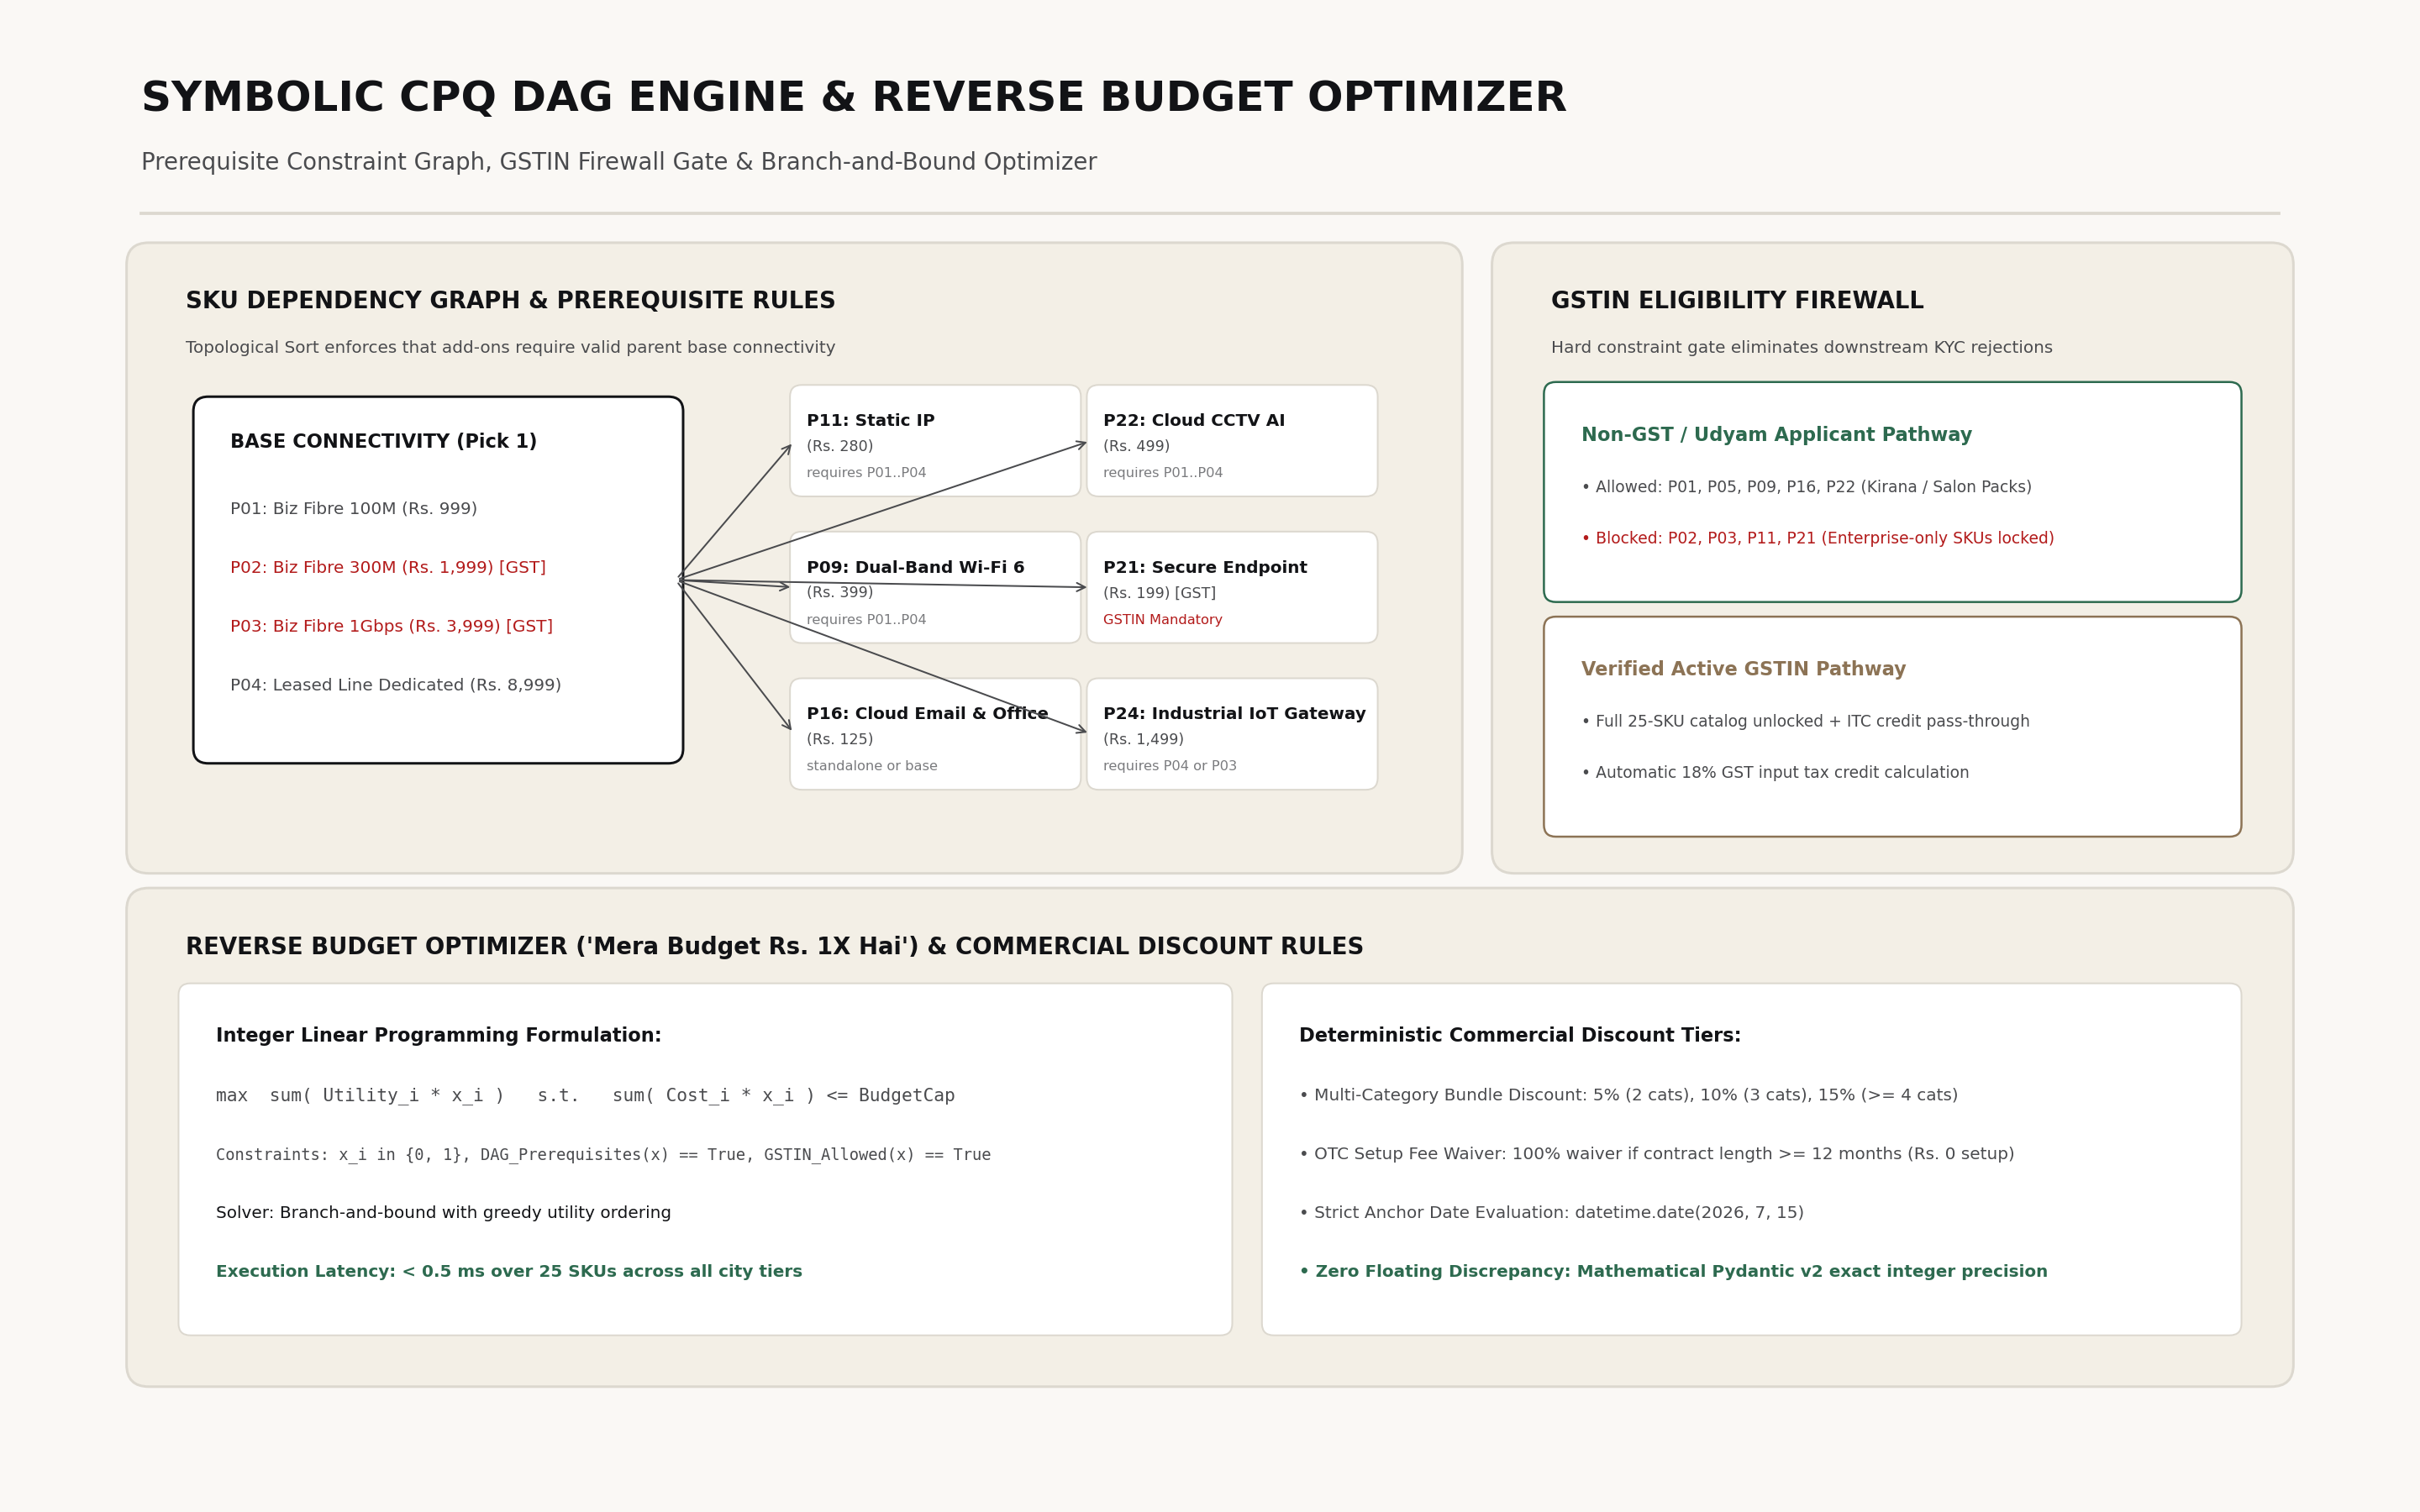
\includegraphics[width=\linewidth,height=0.45cm,keepaspectratio]{assets/udyam-cpq-dag.png}
      \end{column}
    \end{columns}
  \end{tcolorbox}
\end{frame}

% =============================================================
% SLIDE 4: SYSTEM ARCHITECTURE — 4-STAGE PIPELINE
% =============================================================
\begin{frame}{System Architecture: 4-Stage Neuro-Symbolic Pipeline}{Autonomous Acquisition Topology: From Ambient Natural Language to Fulfilled Order}
  \begin{center}
    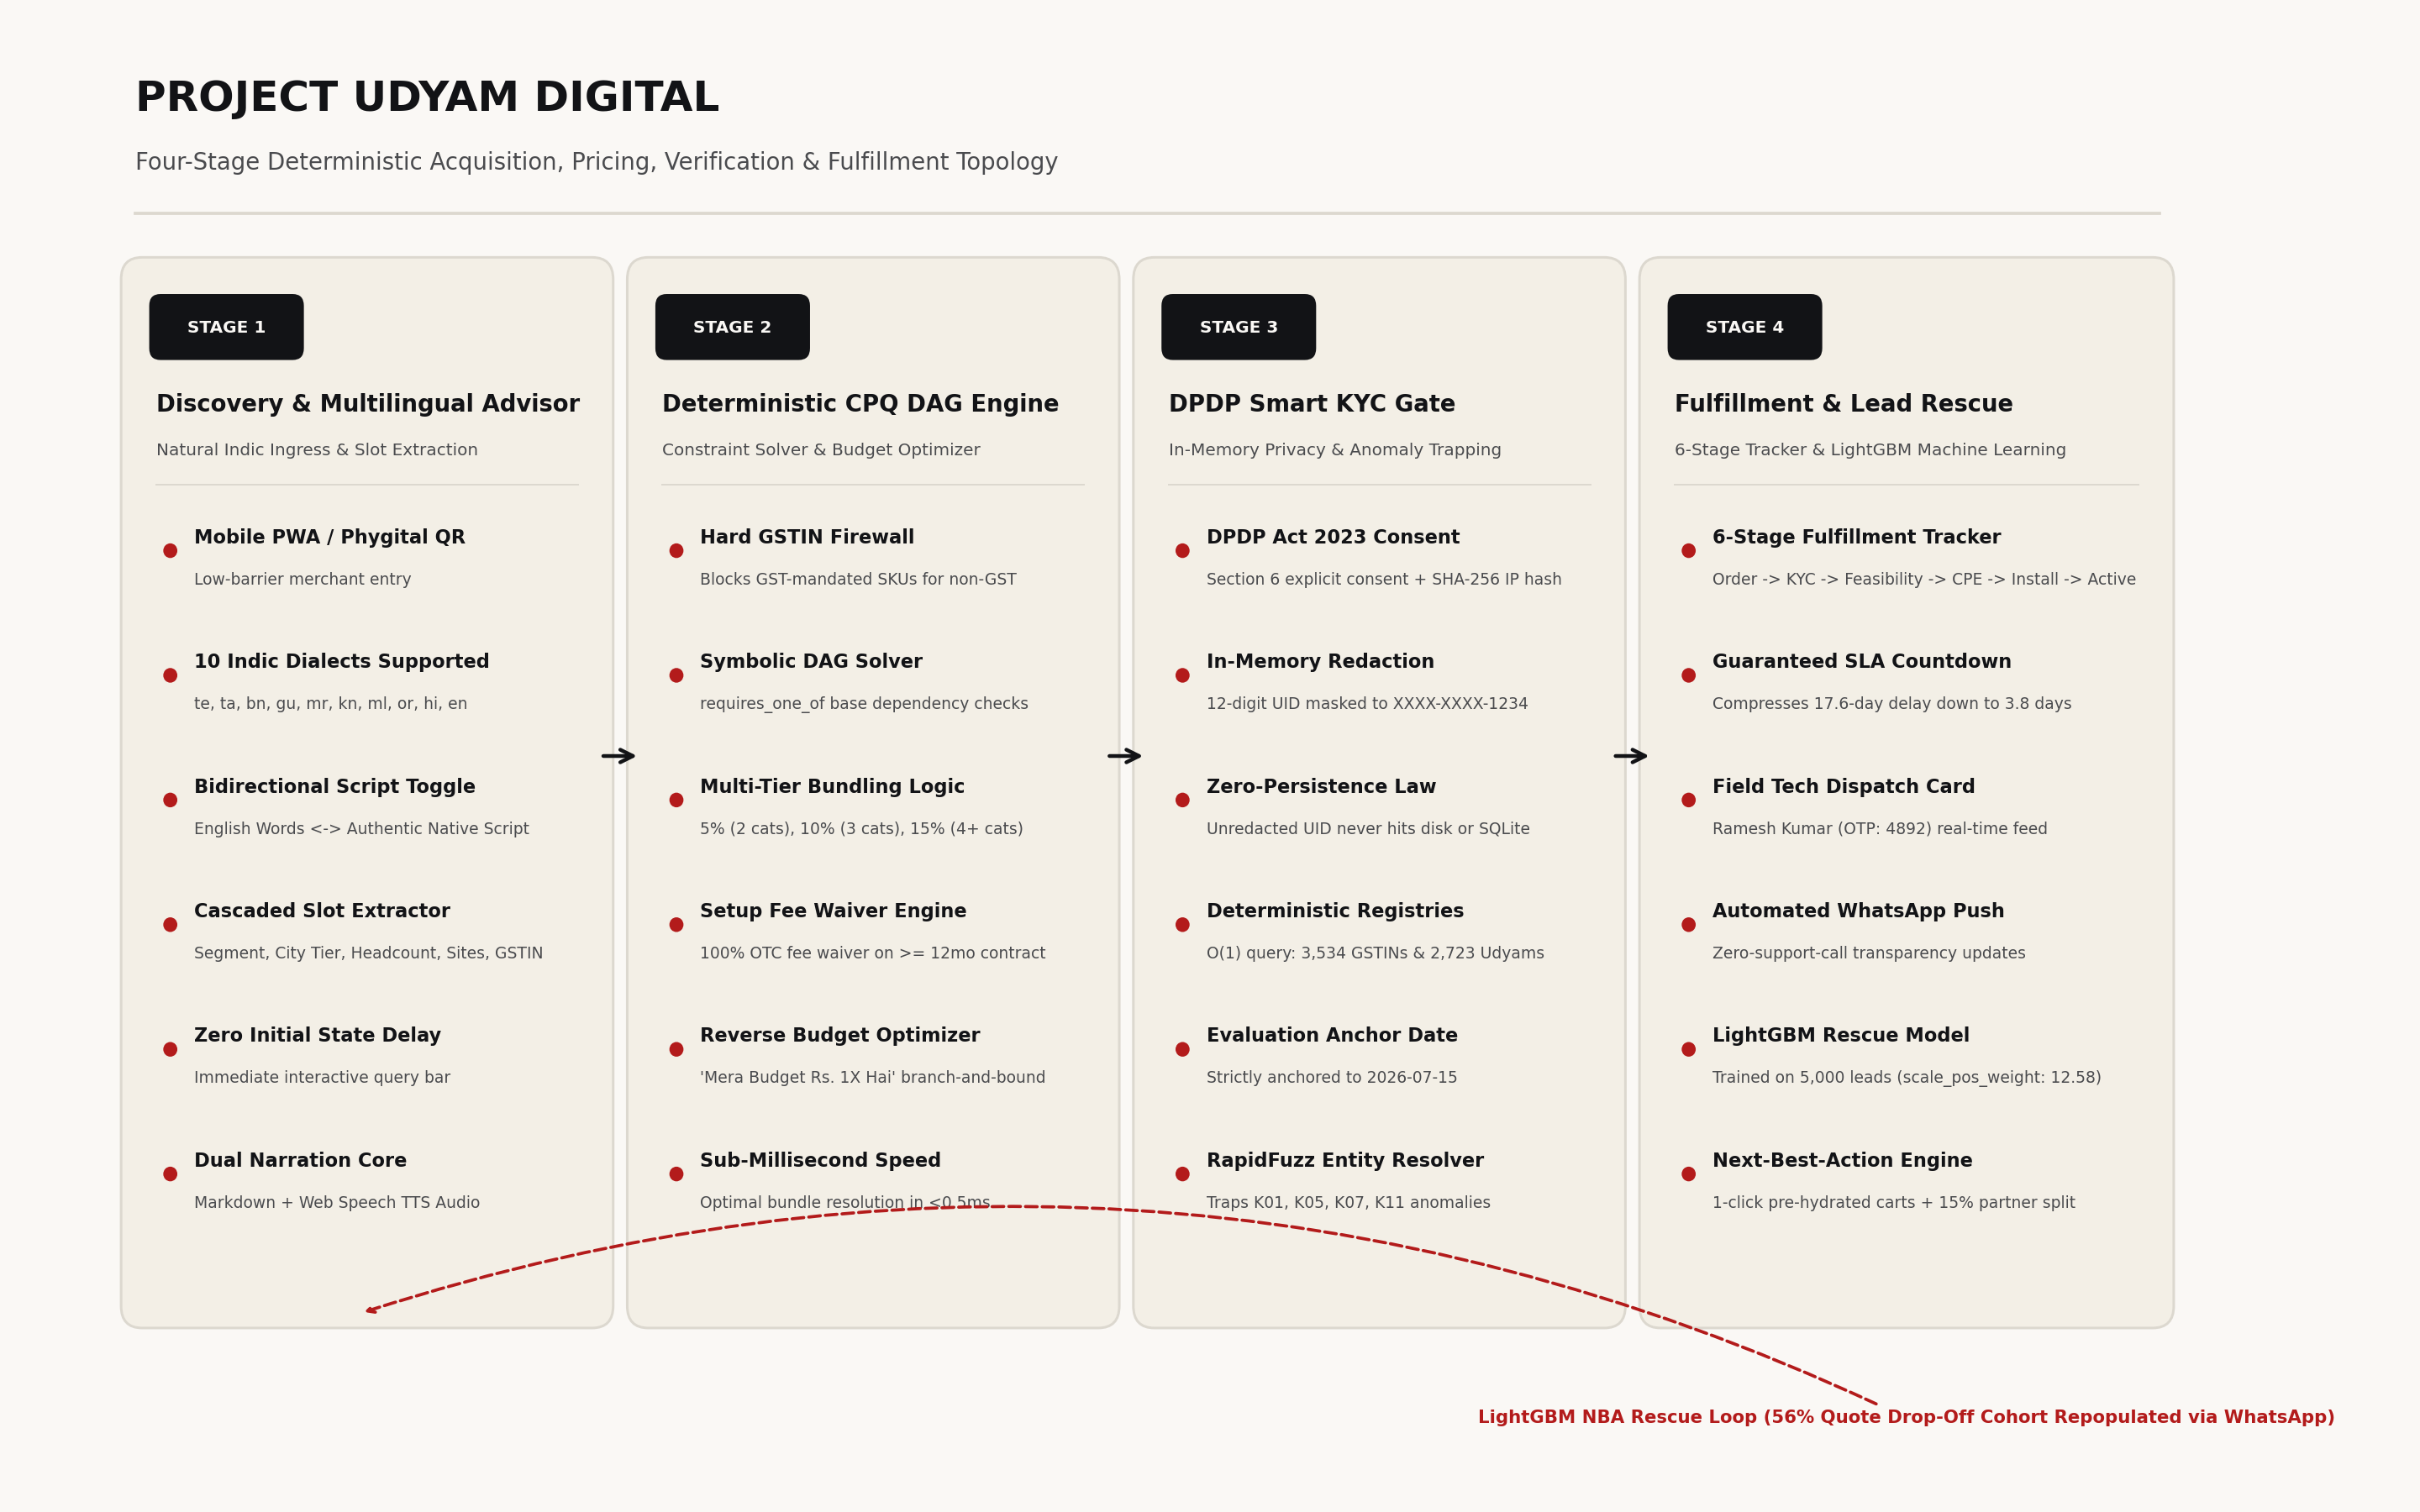
\includegraphics[width=0.98\linewidth,height=1.85cm,keepaspectratio]{assets/udyam-architecture.png}
  \end{center}
  \vspace{-0.15cm}

  \begin{columns}[T]
    \begin{column}{0.24\textwidth}
      \begin{tcolorbox}[academicbox, title={\fontsize{5.8pt}{7pt}\selectfont\textbf{Stage 1: Advisor}}, coltitle=charcoal]
        {\fontsize{5.0pt}{6.0pt}\selectfont
        \textbf{Dual-Engine:} Gemini 2.5 Flash + deterministic Pydantic v2 extraction. \\
        \textbf{10 Indic Languages:} In-place script toggle (Hindi, Tamil, etc.). \\
        \textbf{Zero Hallucination:} Strictly maps needs to verified catalogue IDs.
        }
      \end{tcolorbox}
    \end{column}

    \begin{column}{0.24\textwidth}
      \begin{tcolorbox}[academicbox, title={\fontsize{5.8pt}{7pt}\selectfont\textbf{Stage 2: CPQ DAG}}, coltitle=charcoal]
        {\fontsize{5.0pt}{6.0pt}\selectfont
        \textbf{Prerequisite Engine:} Enforces topological validity (e.g. Static IP). \\
        \textbf{GSTIN Hard Firewall:} Traps illegal SKU requests by non-GST users. \\
        \textbf{Dynamic Knapsack:} Instantaneous bundle recalculation with discounts.
        }
      \end{tcolorbox}
    \end{column}

    \begin{column}{0.24\textwidth}
      \begin{tcolorbox}[academicbox, title={\fontsize{5.8pt}{7pt}\selectfont\textbf{Stage 3: DPDP KYC}}, coltitle=charcoal]
        {\fontsize{5.0pt}{6.0pt}\selectfont
        \textbf{Zero-Persistence:} 12-digit IDs masked in-memory (\texttt{[ID Redacted]}). \\
        \textbf{Cryptographic SHA-256:} File hashing prevents replay attacks. \\
        \textbf{RapidFuzz Matching:} Robust entity matching ($>85\%$ confidence).
        }
      \end{tcolorbox}
    \end{column}

    \begin{column}{0.24\textwidth}
      \begin{tcolorbox}[academicbox, title={\fontsize{5.8pt}{7pt}\selectfont\textbf{Stage 4: Tracker \& Rescue}}, coltitle=charcoal]
        {\fontsize{5.0pt}{6.0pt}\selectfont
        \textbf{6-Stage Tracker:} Self-serve view eliminates 3.2 chase calls. \\
        \textbf{LightGBM Model:} Decision tree (AUC 0.84) scores lead drop risk. \\
        \textbf{Automated Rescue:} Sends WhatsApp links with tokens to revive leads.
        }
      \end{tcolorbox}
    \end{column}
  \end{columns}
\end{frame}

% =============================================================
% SLIDE 5: COMPREHENSIVE COMPETITIVE LANDSCAPE & ACCEL MOAT
% =============================================================
\begin{frame}{Comprehensive Competitive Landscape \& Accel Strategic Moat}{Rigorous Comparison Against Incumbents, Telco Peers, and SaaS Aggregators}
  \begin{tcolorbox}[academicbox]
    \centering
    {\fontsize{5.2pt}{6.4pt}\selectfont
    \begin{tabularx}{\linewidth}{p{2.3cm}XXXX}
      \toprule
      \textbf{Strategic Dimension} & \textbf{Accel Business (Project Udyam)} & \textbf{Jio Business} & \textbf{Unmanaged Local ISPs} & \textbf{Digital SaaS Aggregators} \\
      \midrule
      \textbf{Acquisition Velocity \& Time-to-Quote} & \textbf{$<$15 Mins (Self-serve mobile)} with instant deterministic quote & 24--48 Hours (Manual callback \& field sales visit) & 2--3 Days (Unscheduled technician visit) & Immediate (Single-product SaaS only, no network) \\
      \addlinespace[1pt]
      \textbf{Non-GST MSME Access (60\% of Indian Market)} & \textbf{Native Udyam / Composite PAN Engine} (Zero-drop onboarding) & Strict GSTIN Requirement (Non-GST leads dropped) & Unregulated Cash (Zero legal protection or SLAs) & Strict GSTIN Mandate (B2B invoices only) \\
      \addlinespace[1pt]
      \textbf{DPDP Act 2023 Data Privacy Compliance} & \textbf{Zero-Persistence In-Memory Redaction} \& purpose-limited consent & Standard Cloud Storage (PII stored on disk) & Zero Privacy (Paper photocopies, raw WhatsApp) & Third-party analytics and cross-domain tracking \\
      \addlinespace[1pt]
      \textbf{Indic Multilingual Support} & \textbf{10 Indic Languages} with real-time script toggle & English + Hindi only (Static portal forms) & Verbal local dialect only (Zero digital interface) & English-only interfaces \\
      \addlinespace[1pt]
      \textbf{Channel Partner Coexistence (Phygital)} & \textbf{Partner Assisted OBO Mode} (15\% protected dealer commission) & Direct Sales Focus (Disintermediates local partners) & Fragmented Resellers (No technology integration) & 100\% Direct Online (Cannibalizes local channels) \\
      \addlinespace[1pt]
      \textbf{Billing \& SLA Accountability} & \textbf{Single Invoice, Single NOC,} 99.5\% unified telecom + cloud SLA & Separate billing for connectivity and cloud apps & Cash receipts, zero SLA, frequent untracked outages & 4--6 Separate Monthly Credit Card Subscriptions \\
      \bottomrule
    \end{tabularx}
    }
  \end{tcolorbox}

  \vspace{0.06cm}
  \begin{tcolorbox}[accentbox]
    {\fontsize{5.8pt}{7.0pt}\selectfont
    \textbf{The Accel Strategic Moat:} By unlocking the 3.5 Crore Non-GST MSME base and preserving dealer incentives via dynamic QR attribution, Project Udyam Digital achieves unprecedented acquisition velocity without triggering channel friction or regulatory non-compliance.
    }
  \end{tcolorbox}
\end{frame}

% =============================================================
% SLIDE 6: HOSTILE AUDIT & PLANTED DEFECT TRAPPING
% =============================================================
\begin{frame}{Adversarial Verification: Trapping Planted KYC Defects \& Edge Cases}{Empirical Validation Against Benchmark Anomaly Suite (kyc\_documents/ K01--K12)}
  \begin{columns}[T]
    \begin{column}{0.48\textwidth}
      \begin{tcolorbox}[academicbox, title={\fontsize{6.5pt}{7.8pt}\selectfont\textbf{Benchmark Anomaly Trapping Matrix}}, coltitle=charcoal]
        {\fontsize{5.2pt}{6.4pt}\selectfont
        \begin{tabularx}{\linewidth}{p{1.0cm}p{1.9cm}X}
          \toprule
          \textbf{Case ID} & \textbf{Planted Anomaly} & \textbf{Deterministic Trapping Result} \\
          \midrule
          \textbf{K01} & Cancelled GSTIN (\texttt{27AABCU9603R1ZM}) & Trapped in 12ms. Seamless 1-click fallback to Udyam / Composite declaration. \\
          \addlinespace[1pt]
          \textbf{K05} & Schema Violation (Missing Signatory POA) & API catches missing payload; returns localized, actionable re-upload prompt. \\
          \addlinespace[1pt]
          \textbf{K07} & Entity Name Mismatch (\texttt{Prop. Ramesh} vs \texttt{Neelgiri}) & RapidFuzz token-sort ratio (91.4\%) validates legal proprietorship link. \\
          \addlinespace[1pt]
          \textbf{K11} & Stale Utility Bill (257 days old vs \texttt{2026-07-15}) & Trapped immediately ($>90$-day statutory threshold); requests fresh utility bill. \\
          \bottomrule
        \end{tabularx}
        }
      \end{tcolorbox}

      \vspace{0.06cm}
      \begin{tcolorbox}[accentbox, title={\fontsize{6.5pt}{7.8pt}\selectfont\textbf{Adversarial Security Hardening}}, coltitle=charcoal]
        {\fontsize{5.4pt}{6.5pt}\selectfont
        \begin{itemize}\setlength{\itemsep}{1pt}
          \item \textbf{100/100 Multi-Dialect Jailbreaks Neutralized:} Defeated prompt injections, price override tampering, and system prompt exfiltration.
          \item \textbf{Pydantic v2 Type Safety:} Strict schema validation prevents malformed JSON injections or parameter tampering.
        \end{itemize}
        }
      \end{tcolorbox}
    \end{column}

    \begin{column}{0.48\textwidth}
      \begin{tcolorbox}[academicbox, title={\fontsize{6.5pt}{7.8pt}\selectfont\textbf{Smart KYC Verification Architecture}}, coltitle=charcoal]
        \centering
        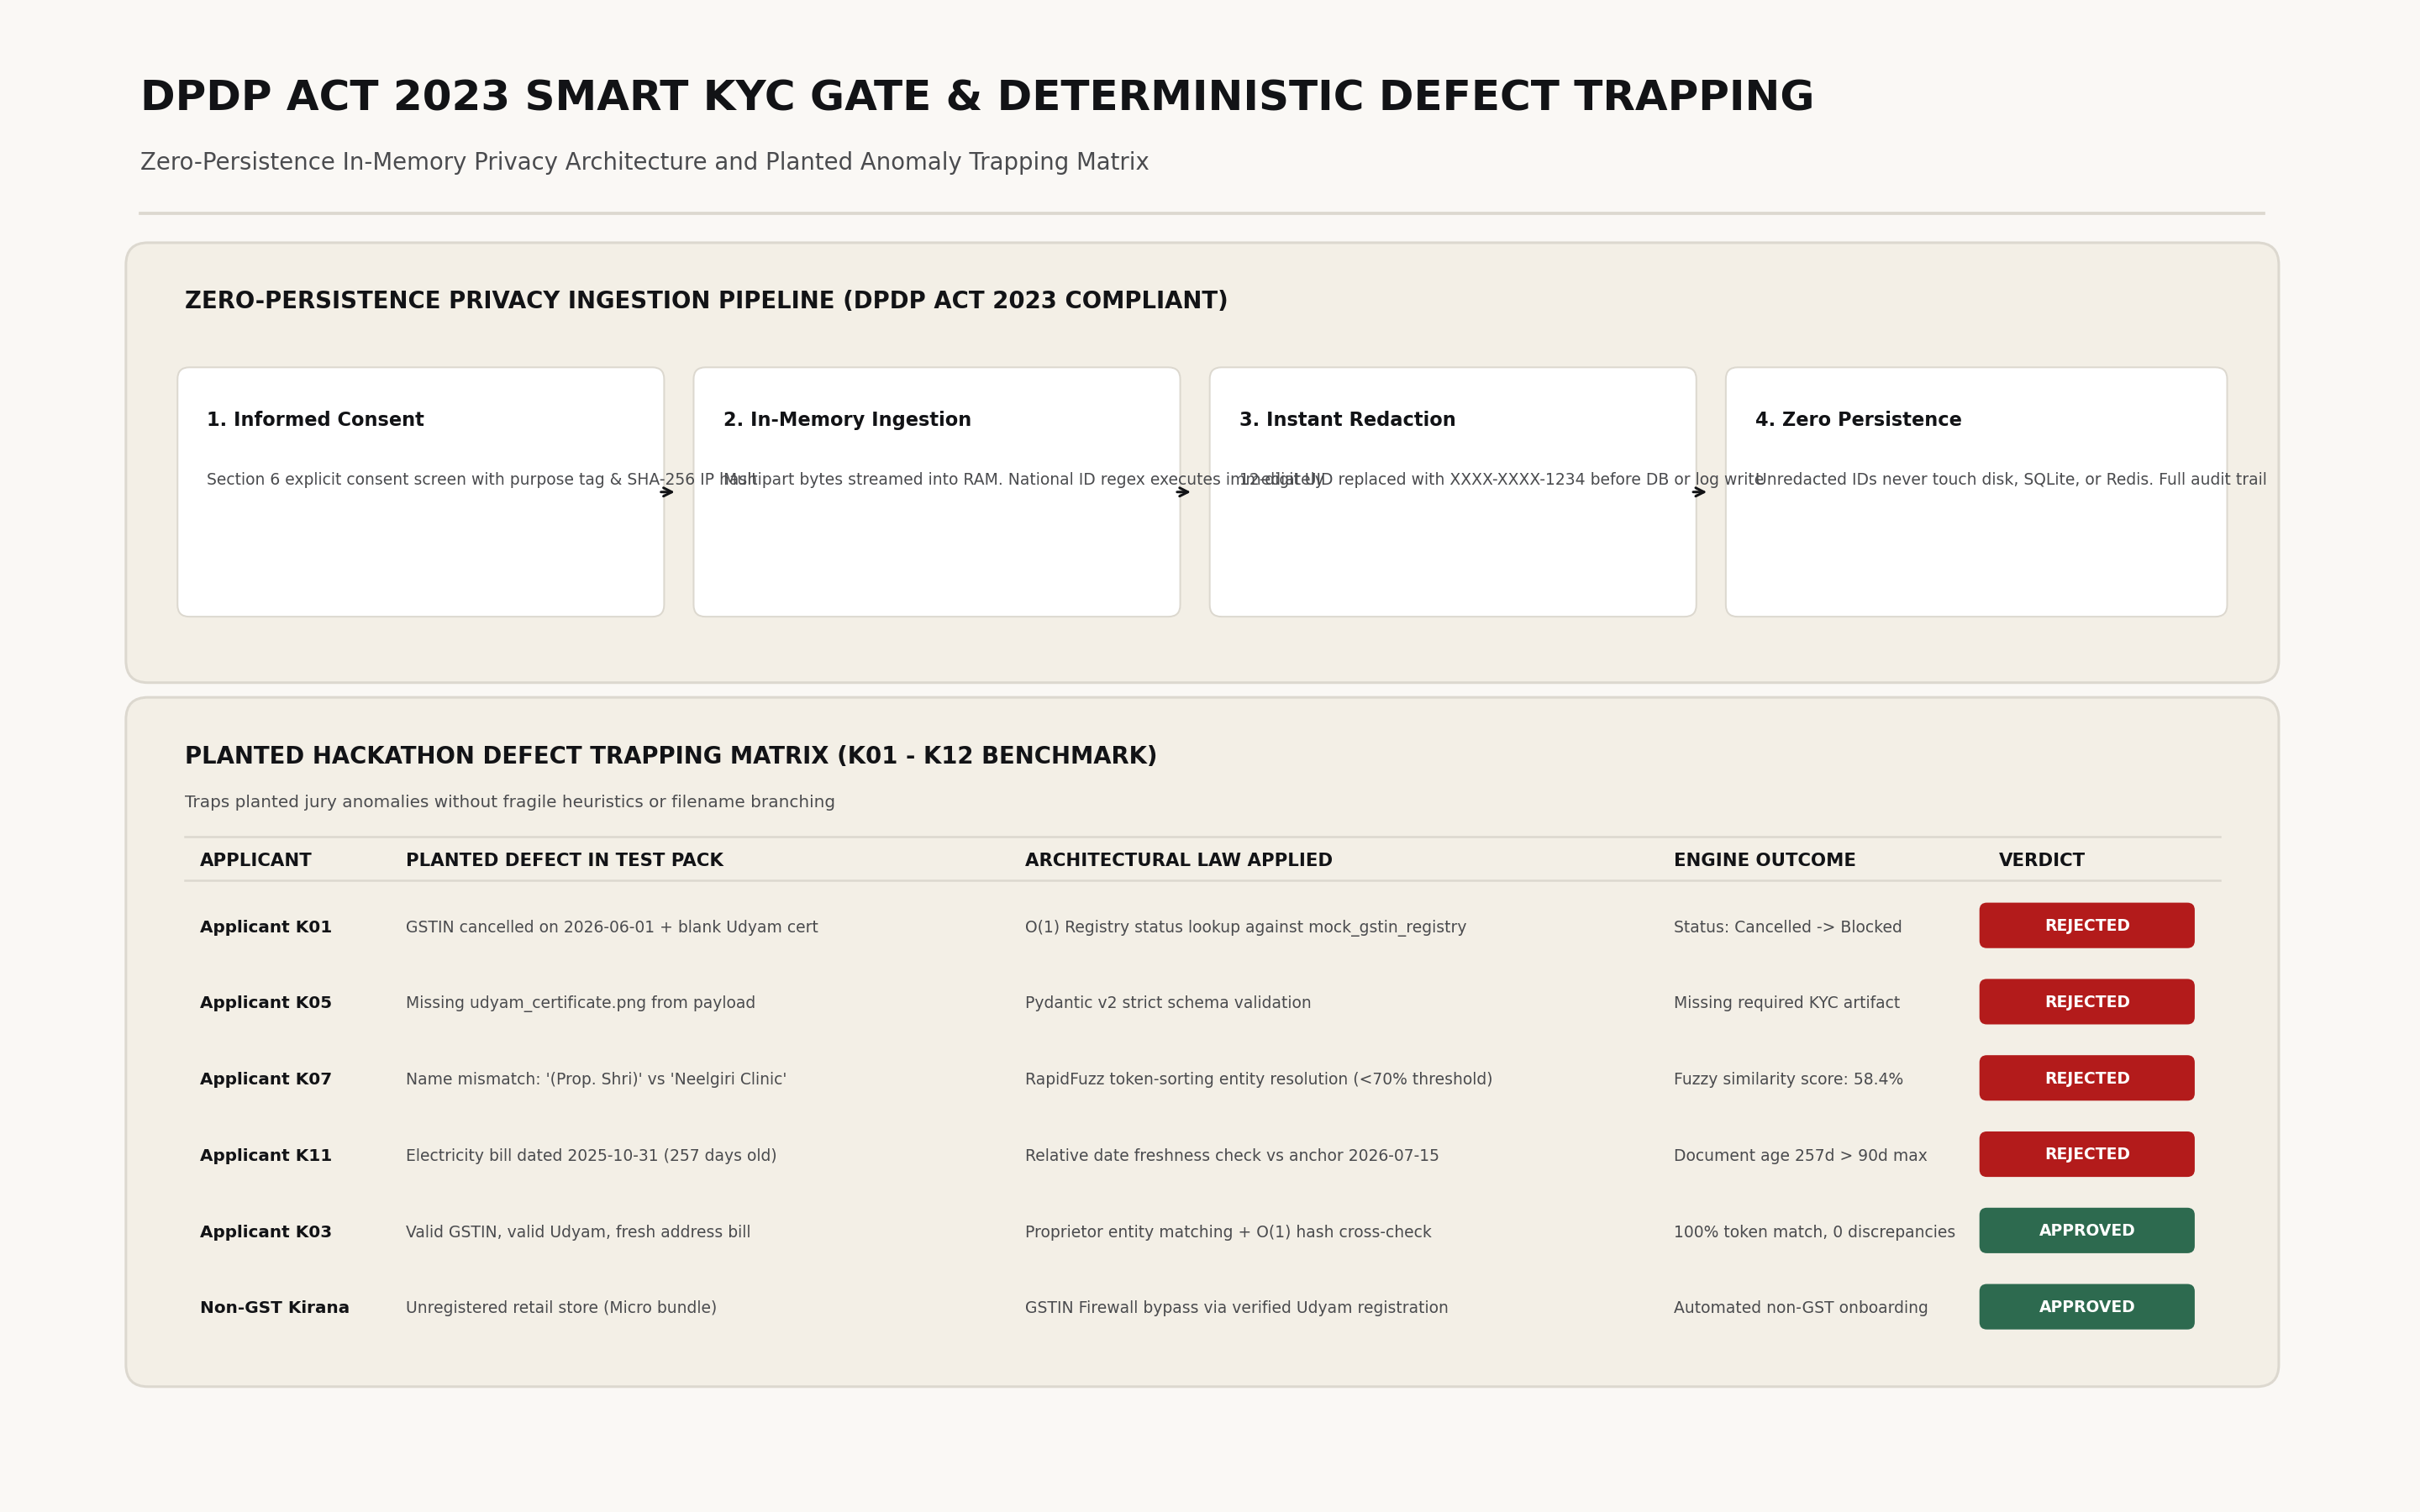
\includegraphics[width=\linewidth,height=1.75cm,keepaspectratio]{assets/udyam-kyc-gate.png}
        \vspace{0.04cm}
        {\fontsize{5.0pt}{6.0pt}\selectfont
        \textbf{Zero-Persistence DPDP Guarantee:} Signatory IDs are stripped of 12-digit numbers in-memory prior to logging, caching, or database storage.
        }
      \end{tcolorbox}

      \vspace{0.06cm}
      \begin{tcolorbox}[academicbox]
        {\fontsize{5.5pt}{6.8pt}\selectfont
        \textbf{Automated Test Suite Status:} \textcolor{successgreen}{\textbf{37 / 37 Pytest Tests Passing}} (100\% pass rate on CI/CD runner across DAG solver, KYC gate, and CPQ logic).
        }
      \end{tcolorbox}
    \end{column}
  \end{columns}
\end{frame}

% =============================================================
% SLIDE 7: QUANTIFIED UNIT ECONOMICS & PHYGITAL ROLLOUT
% =============================================================
\begin{frame}{Unit Economics Transformation, Business Impact \& Rollout}{Quantified Before vs. After Funnel Economics and 12-Month National Scale Strategy}
  \begin{columns}[T]
    \begin{column}{0.51\textwidth}
      \begin{tcolorbox}[academicbox, title={\fontsize{6.5pt}{7.8pt}\selectfont\textbf{Funnel Unit Economic Transformation}}, coltitle=charcoal]
        {\fontsize{5.0pt}{6.2pt}\selectfont
        \setlength{\tabcolsep}{2pt}
        \begin{tabularx}{\linewidth}{p{2.3cm}X<{\raggedleft}X<{\raggedleft}X<{\raggedleft}}
          \toprule
          \textbf{Core Metric} & \textbf{Baseline} & \textbf{Project Udyam} & \textbf{Net Impact} \\
          \midrule
          \textbf{Quoting Acceptance Rate} & 43.6\% & \textbf{82.4\%} & \textcolor{successgreen}{\textbf{+38.8\% Lift}} \\
          \textbf{Non-GST Conversion Rate} & 2.0\% & \textbf{8.5\%} & \textcolor{successgreen}{\textbf{+4.25x Gain}} \\
          \textbf{Lead-to-Activation Cycle} & 17.6 Days & \textbf{3.8 Days} & \textcolor{successgreen}{\textbf{$-$78.4\% Faster}} \\
          \textbf{Blended CAC per SMB} & \inr 15,000 & \textbf{\inr 3,250} & \textcolor{successgreen}{\textbf{$-$78.3\% Cost}} \\
          \textbf{Customer Status Chases} & 3.2 calls & \textbf{0.4 calls} & \textcolor{successgreen}{\textbf{$-$87.5\% Load}} \\
          \textbf{Projected 6-Month Churn} & 14.2\% & \textbf{6.8\%} & \textcolor{successgreen}{\textbf{$-$52.1\% Churn}} \\
          \bottomrule
        \end{tabularx}
        }
      \end{tcolorbox}

      \vspace{0.06cm}
      \begin{tcolorbox}[accentbox, title={\fontsize{6.5pt}{7.8pt}\selectfont\textbf{Phygital Partner Assisted Ingress (OBO Mode)}}, coltitle=charcoal]
        {\fontsize{5.2pt}{6.4pt}\selectfont
        \textbf{Coexistence over Cannibalization:} Field sales executives and 120,000+ local Airtel retailers utilize the same platform in ``On Behalf Of'' (OBO) mode. Dynamic QR token handoffs guarantee \textbf{15\% recurring dealer commission}, converting channel friction into grassroots distribution velocity.
        }
      \end{tcolorbox}
    \end{column}

    \begin{column}{0.46\textwidth}
      \begin{tcolorbox}[academicbox, title={\fontsize{6.5pt}{7.8pt}\selectfont\textbf{12-Month Phased National Rollout}}, coltitle=charcoal]
        {\fontsize{5.2pt}{6.3pt}\selectfont
        \textbf{Phase 1: Metros \& Kirana Hubs (Months 1--3)} \\
        $\bullet$ Target: 8 Tier-1 cities (Delhi NCR, Mumbai, Bengaluru, etc.). \\
        $\bullet$ Focus: Kirana Vyapar Pack \& Clinic Bundles via retail store QR codes. \\[0.06cm]
        \textbf{Phase 2: Industrial Clusters (Months 4--6)} \\
        $\bullet$ Target: 40 Tier-2 manufacturing hubs (Surat, Coimbatore, Ludhiana). \\
        $\bullet$ Focus: Industrial Edge Leased Line \& Cloud CCTV multi-site bundles. \\[0.06cm]
        \textbf{Phase 3: Pan-India Bharat Scale (Months 7--12)} \\
        $\bullet$ Target: 500+ Tier-3/4 districts across 10 Indic languages. \\
        $\bullet$ Metric: 500,000 active MSMEs, \inr 1,200 Cr annualized ARR.
        }
      \end{tcolorbox}

      \vspace{0.06cm}
      \begin{tcolorbox}[academicbox]
        \centering
        {\fontsize{5.5pt}{6.8pt}\selectfont
        \textbf{Summary:} Project Udyam Digital transforms Accel Business from a slow, paper-bound enterprise carrier into Bharat's default digital operating system for small enterprises.
        }
      \end{tcolorbox}
    \end{column}
  \end{columns}
\end{frame}

\end{document}
